\documentclass[conference]{IEEEtran}
\usepackage[T1]{fontenc}
\usepackage[utf8]{inputenc}
\usepackage{graphicx}
\usepackage{booktabs}
\usepackage{array}
\usepackage{multirow}
\usepackage{hyperref}
\usepackage{xcolor}
\usepackage{enumitem}
\usepackage{amsmath}
\usepackage{tabularx}
\usepackage{float}
\usepackage{caption}
\hypersetup{hidelinks}
\graphicspath{{../../modelling/99_model_comparison/results/plots}}

\title{Bike Rental Demand Forecasting\\From Data Preparation to Model Comparison and Critical Reflection}

\author{
\IEEEauthorblockN{Anton Wilhelmi and Alexander Harant}
\IEEEauthorblockA{Introduction to Machine Learning\\
Group Project - Deliverable 2}
}

\begin{document}
\maketitle

\begin{abstract}
This report documents the full workflow after the first problem formulation and integrates the earlier data preparation summary into one continuous methodological story. We explain how the raw bike rental data was reduced to a clean modelling table, why each transformation was made, how the regression pipeline was built, which models were trained, how they were evaluated, and what the current results mean. The final reduced dataset contains one target, \texttt{total\_rentals}, and 17 numeric predictors. We then compared eight regression models with the same chronological train-validation-test split and the same evaluation metrics. The comparison shows that ensemble tree methods currently perform best: Gradient Boosting is the best validation model, while Random Forest is the best model on the held-out test set. At the same time, the results also show clear weaknesses in the current representation, especially the limited treatment of station identity and time structure. We therefore end the report with a critical discussion of what still limits the system and what should be improved next.
\end{abstract}

\section{Introduction}
The goal of the project is to predict bike rental demand with machine learning in a way that is 
technically sound, reproducible, and easy to justify.

This report therefore combines two pieces of work into one coherent document. First, it includes 
the complete reasoning behind the final reduced dataset, because the modelling results only make 
sense if the data representation is clear. Second, it describes the modelling pipeline that starts 
from this reduced dataset and compares several regression models under the same evaluation protocol.

\section{From Deliverable 1 to Deliverable 2}
The first deliverable framed the task as bike rental demand forecasting and already highlighted 
several relevant ideas: the problem is a regression problem, the target should be a rental count, 
time-aware splitting is necessary, and leakage variables must be removed. These ideas stayed central 
in the second phase.

However, after the first deliverable we also made important adjustments. The main change is that we 
built a much more explicit data processing pipeline. Instead of directly going from raw data to 
modelling, we first created a structured daily station-level dataset, analysed feature redundancy, 
simplified the target, and produced one final numeric modelling table. This adjustment was necessary 
because a clean input representation is the basis of a fair model comparison.

We extended the evaluation to MAE, RMSE, median absolute error, MAPE, $R^2$, and explained variance. 
This gives a much more complete view of model behaviour.

A third change is that we built a shared project structure for modelling. All models now use the 
same common utilities, the same split logic, the same target, and the same output structure. This 
makes the experiments easier to compare and also reduces the risk that one model appears better 
only because it was run under a different setup.

\section{Data Preparation Methodology}
\subsection{Why we reduced the raw data}
The raw data was delivered in four files contained detailed rental data, station information, usage frequency data, and weather 
data. Working with the raw tables directly would have made the modelling phase harder to interpret and 
more error-prone. Therefore, the first goal was to build one clean analytical table 
that could later be used for regression.

We decided to focus on the 20 most used start stations. This was a practical and methodological decision. 
Practically, it reduced the size of the problem (2,8 GB file) and made early experimentation faster. Methodologically, 
it also reduced noise from stations with very few observations. Rare stations can introduce unstable 
patterns, while highly used stations provide a stronger and more consistent signal. The idea was not 
to claim that rare stations are unimportant, but to create a stable first forecasting setup before 
scaling the problem further.

The next step was to aggregate the rental information at daily station level and merge it with weather 
variables. This aggregation created a table where every row corresponds to one station-day combination. 
This step was important because it aligned the demand outcome with the explanatory variables we wanted 
to use. If weather is available daily, then a daily demand representation is also a natural first 
modelling level.

\subsection{Why we stored station names separately}
At one stage the processed data still contained both \texttt{start\_station\_id} and station names. 
We removed the name columns from the modelling table and stored the mapping in a separate file. The 
reason is simple: station names are descriptive labels for humans, but they do not add predictive 
information beyond the station identifier. Keeping both inside the modelling matrix would only duplicate 
the same information and make the dataset less clean.

This decision also made later steps easier. The modelling table stays compact and numeric, while the 
mapping file still allows us to interpret results by station when needed.

\subsection{Why we changed the date representation}
The raw date column was not kept in its original form in the final modelling file. A string-based date 
is not directly useful for the regression models we trained. Instead of leaving the raw date string in 
the table, we represented time through numeric variables such as month, weekday, year 
and a chronological index called \texttt{time\_idx}.

This decision had two advantages. First, the final input matrix became directly trainable because 
all predictors were numeric. Second, we did not lose the time structure of the data. The new variables 
still preserve seasonality and order, but in a format that the models can process.

\subsection{Why we analysed correlations before modelling}
Before creating the final reduced dataset, we computed a correlation matrix and a heatmap for the 
predictors. The purpose was to identify variables that carried almost the same information. 
This matters because redundant predictors can make models less stable and harder to interpret. 
The issue is especially relevant for linear models, where strong collinearity can distort coefficients.

The analysis showed that several weather variables were nearly duplicates. Examples included:\newline
\texttt{solarenergy} vs. \texttt{solarradiation},\newline
\texttt{feelslike} vs. \texttt{temp},\newline
\texttt{feelslikemin} vs. \texttt{tempmin},\newline
\texttt{feelslikemax} vs. \texttt{tempmax}.

We kept the more interpretable or slightly more informative variable and removed the weaker duplicate. 
This reduced unnecessary redundancy and made the final dataset easier to explain. We did not try to 
remove every possible relationship between predictors, because some correlation is natural in weather 
data, but we removed the strongest near-duplicates that offered almost no new information.

\subsection{Why we simplified the target to one output}
During preprocessing, the dataset still contained multiple rental-related count columns, for example 
counts for members and casual users or counts for specific bike types. At first glance these columns 
look useful, but they create a serious modelling problem when the main prediction target 
is \texttt{total\_rentals}. The reason is that these sub-counts are structurally tied to the 
total and may allow the model to reconstruct the answer almost directly.

To avoid this issue, we removed the count decomposition and kept only one target variable:
\begin{center}
\texttt{total\_rentals}
\end{center}

This was a very important decision. It turned the task into one clean regression problem and 
avoided a leakage-like situation in which the model would partly learn the target from variables 
that are conceptually too close to it.

\subsection{Why we did not apply PCA}
We also considered whether a PCA-based representation would be useful. We decided against it. After 
the correlation-based reduction, the number of predictors was already manageable. PCA would have 
transformed the remaining features into mixtures of original variables, which would make the model 
harder to interpret. Since this project strongly values explainability and critical reflection, 
preserving the meaning of the original predictors was more valuable than compressing them further.

\subsection{Final reduced dataset}
The final modelling table contains one target and 17 predictors. The predictors are:
\begin{quote}
\small
\texttt{start\_station\_id}, \texttt{tempmax}, \texttt{humidity}, \texttt{precip}, \texttt{precipcover}, \texttt{cloudcover}, \texttt{windspeed}, \texttt{visibility}, \texttt{sealevelpressure}, \texttt{uvindex}, \texttt{sunset\_minutes}, \texttt{month}, \texttt{weekday}, \texttt{year}, \texttt{time\_idx}, \texttt{snow}, \texttt{snowdepth}
\end{quote}

This final dataset is compact, fully numeric, and directly usable for machine learning. It is also 
the direct result of several explicit design decisions rather than an arbitrary column selection.

\section{Modelling Pipeline After Data Preparation}
\subsection{Why we created a shared modelling structure}
Once the final dataset was ready, we built a structured \texttt{modelling} folder. Each model has its 
own subfolder, and all common functionality is stored in a \texttt{common} folder. This decision was 
made for reproducibility, consistency, and easier debugging.

The \texttt{common} folder contains the shared code for paths and settings, preprocessing, splitting, 
metrics, plotting, and file saving. This means that every model script follows the same core logic: 
load the same reduced dataset, build the same time-aware split, predict the same target, compute the 
same metrics, and save outputs in the same format. This matters because a model comparison is only 
fair if the evaluation procedure is consistent.

\subsection{Why we used a chronological split}
We used a chronological split with 70\% training data, 15\% validation data, and 15\% test data. 
We did not use a random split. This is one of the most important methodological decisions in the report.

The reason is that bike demand is a time-based problem. In a real forecasting scenario, a model is 
trained on older data and then asked to predict future demand. A random split would mix older and 
newer observations and would therefore make the problem unrealistically easy. It could also create 
information leakage across time. The chronological split respects the natural order of the 
observations and produces a more honest estimate of future performance.

The variable \texttt{time\_idx} was used to maintain the exact order of the station-day observations. 
Because the split is stricter than a random split, the resulting scores are harder to optimize, 
but they are also much more realistic.

\subsection{Why we scaled only selected models}
Feature scaling was applied only where it is methodologically appropriate. Linear models, regularized 
linear models, and KNN are sensitive to feature magnitude, so scaling is necessary there. Otherwise a 
feature with a large numeric range can dominate other predictors for purely numerical reasons.

Tree-based models work differently. They split on thresholds and do not depend on Euclidean distance 
or coefficient penalty in the same way. Therefore, scaling is not required for Decision Tree, Random 
Forest, or Gradient Boosting. This selective scaling choice keeps the preprocessing aligned with the 
modelling assumptions.

\section{Model Selection Strategy and Justification}
We deliberately started with simple models and then moved towards more flexible models. This follows 
the lecture logic of establishing a baseline, then adding complexity only when it is justified.

\subsection{Dummy Regressor}
The Dummy Regressor was used as the minimum reference point. It does not learn real relationships 
from the data. Its role is to answer a simple question: do the real models extract useful signal at 
all? If a real model cannot improve over the dummy baseline, then either the representation is too 
weak or the modelling setup is flawed.

\subsection{Linear Regression}
Linear Regression was the first real predictive model because it is easy to interpret and acts as a 
clean benchmark. It tells us whether the final reduced features already contain a meaningful 
approximately linear signal. It is also a good diagnostic model because poor performance here can 
reveal weak representation or strong nonlinearity.

\subsection{Ridge Regression}
Ridge Regression extends Linear Regression by shrinking coefficients. This is useful when predictors 
are still somewhat correlated, which is likely in weather and calendar data. The reason for including 
Ridge was therefore not only performance but also stability. If Ridge improves over plain Linear 
Regression, that is evidence that mild regularization is helpful.

\subsection{Lasso Regression}
Lasso was included because it regularizes even more aggressively and can shrink some coefficients 
toward zero. This makes it useful when we suspect that not all predictors are equally helpful. Lasso 
therefore adds a feature-selection perspective on top of regularized regression.

\subsection{Decision Tree}
A Decision Tree was tested because it can model nonlinear interactions and threshold effects without 
requiring manual feature transformations. This is appealing for weather-driven demand, where effects 
are often not purely linear. However, single trees can overfit, so they also serve as a useful 
contrast between interpretability and stability.

\subsection{KNN Regressor}
KNN was included as a local neighbourhood model. The idea behind it is simple: similar observations 
may have similar target values. KNN can capture local structure that linear models miss, but it is 
highly sensitive to scaling and often becomes slower at prediction time. Including it helped us 
compare a distance-based strategy with coefficient-based and tree-based strategies.

\subsection{Random Forest}
Random Forest was a natural next step after Decision Tree. A single tree is flexible but unstable. 
Random Forest reduces this instability by combining many trees trained on bootstrapped samples. It is 
therefore a good candidate when a single tree seems promising but too variable. In course terms, it is 
also a bagging method that can reduce variance.

\subsection{Gradient Boosting}
Gradient Boosting was included because boosting can reduce bias by building trees sequentially and 
focusing on the remaining errors. This makes it a strong candidate when simpler models underfit the 
demand structure. It is typically more powerful than a single tree, but also more computationally 
expensive and more sensitive to hyperparameter choices.

\section{Evaluation Strategy and Metrics}
We used multiple regression metrics because one metric alone would give an incomplete picture.

\textbf{MAE} reports the average absolute error in the original rental units. This is easy to interpret.\newline
\textbf{RMSE} penalizes large errors more strongly than MAE and is therefore useful when large misses are especially problematic.\newline
\textbf{Median Absolute Error} gives a robust estimate of the typical error and is less influenced by extreme values.\newline
\textbf{MAPE} gives a relative error view, which is useful but must be interpreted carefully when actual demand is small.\newline
\textbf{$R^2$} reports how much variance of the target is explained by the model.\newline
\textbf{Explained Variance} adds a second variance-based interpretation and supports the same general idea from a slightly different angle.

Using this metric set is important because different models may look good under one measure and less 
good under another. A model that minimizes RMSE may not be the fastest model or the one with the best 
MAPE. The broader view is therefore more honest.

\section{Results and Model Comparison}
Table~\ref{tab:main-results} summarizes the most relevant validation and test results for all eight models.

\begin{table*}[t]
\caption{Main comparison results for all evaluated models}
\label{tab:main-results}
\centering
\footnotesize
\begin{tabular}{lrrrrrrrr}
\toprule
Model & Val. MAE & Val. RMSE & Val. $R^2$ & Test MAE & Test RMSE & Test $R^2$ & Fit Time (s) & Predict Time (s) \\
\midrule
Dummy             & 37.00 & 46.10 & -0.533 & 38.14 & 48.56 & -0.523 & 0.001 & 0.000 \\
Linear            & 26.14 & 32.94 &  0.217 & 29.40 & 36.72 &  0.129 & 0.018 & 0.002 \\
Ridge             & 25.57 & 32.37 &  0.244 & 28.68 & 35.91 &  0.167 & 0.003 & 0.000 \\
Lasso             & 24.04 & 31.13 &  0.301 & 26.21 & 33.49 &  0.275 & 0.027 & 0.002 \\
Decision Tree     & 21.33 & 28.64 &  0.408 & 24.32 & 32.03 &  0.337 & 0.109 & 0.005 \\
KNN               & 23.50 & 31.14 &  0.301 & 24.42 & 32.35 &  0.324 & 0.001 & 0.832 \\
Random Forest     & 20.40 & 27.28 &  0.463 & 22.87 & 30.31 &  0.406 & 0.872 & 0.185 \\
Gradient Boosting & 20.53 & 27.00 &  0.474 & 23.71 & 30.57 &  0.396 & 6.232 & 0.050 \\
\bottomrule
\end{tabular}
\end{table*}

The first clear result is that all real models outperform the dummy baseline by a large margin. This is 
an important positive finding because it shows that the reduced dataset contains real predictive signal.

The second result is that the linear family improves in a meaningful sequence: Linear Regression is 
clearly better than Dummy, Ridge improves slightly over Linear, and Lasso improves further. This tells 
us that regularization helps, but it also suggests that the demand problem is not purely linear.

The third and strongest result is that the ensemble tree models are currently the best performers. 
Gradient Boosting achieves the best validation RMSE (27.00) and the best validation $R^2$ (0.474), 
while Random Forest achieves the best held-out test RMSE (30.31), the best test MAE (22.87), and the 
best test $R^2$ (0.406). This means that the two strongest models in the current project phase are 
the two ensemble tree methods, with Random Forest currently being the safer final choice because the 
test set is the most important final evaluation set.

\section{Visual Comparison of the Models}

\begin{figure*}[t]
    \centering
    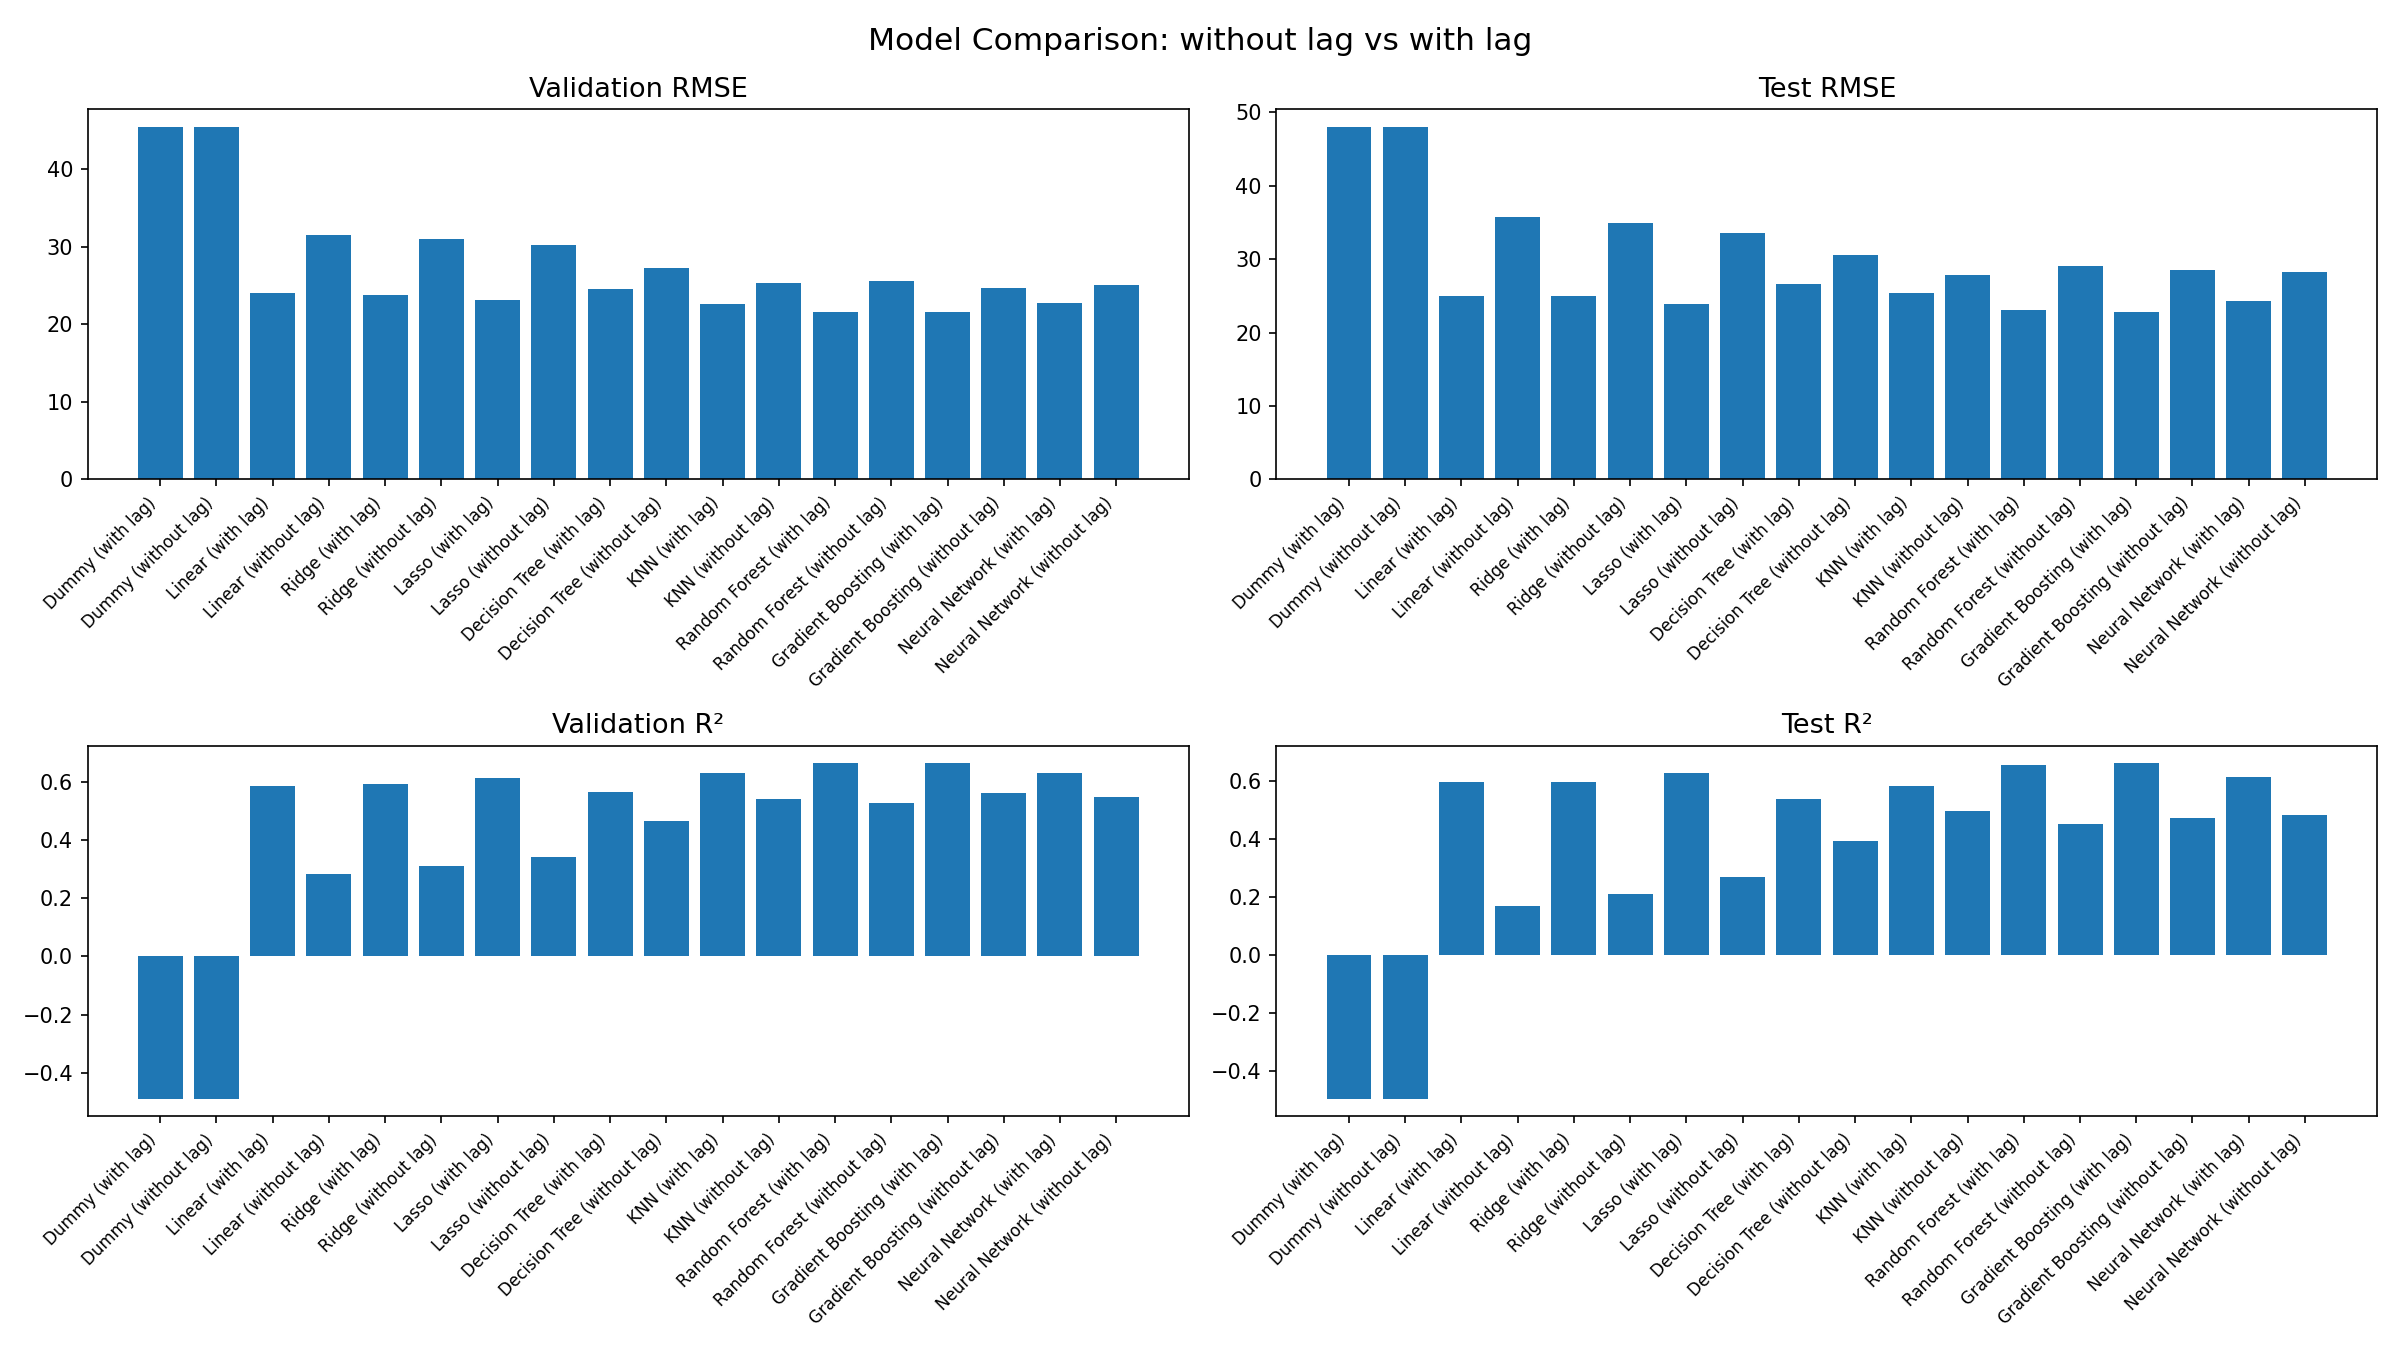
\includegraphics[width=0.95\textwidth]{model_comparison_overview.png}
    \caption{Overview of the most important comparison dimensions. The figure highlights that Gradient Boosting is strongest on validation, while Random Forest is strongest on the held-out test set.}
    \label{fig:overview}
\end{figure*}

\begin{figure}[H]
    \centering
    \begin{minipage}{0.49\textwidth}
        \centering
        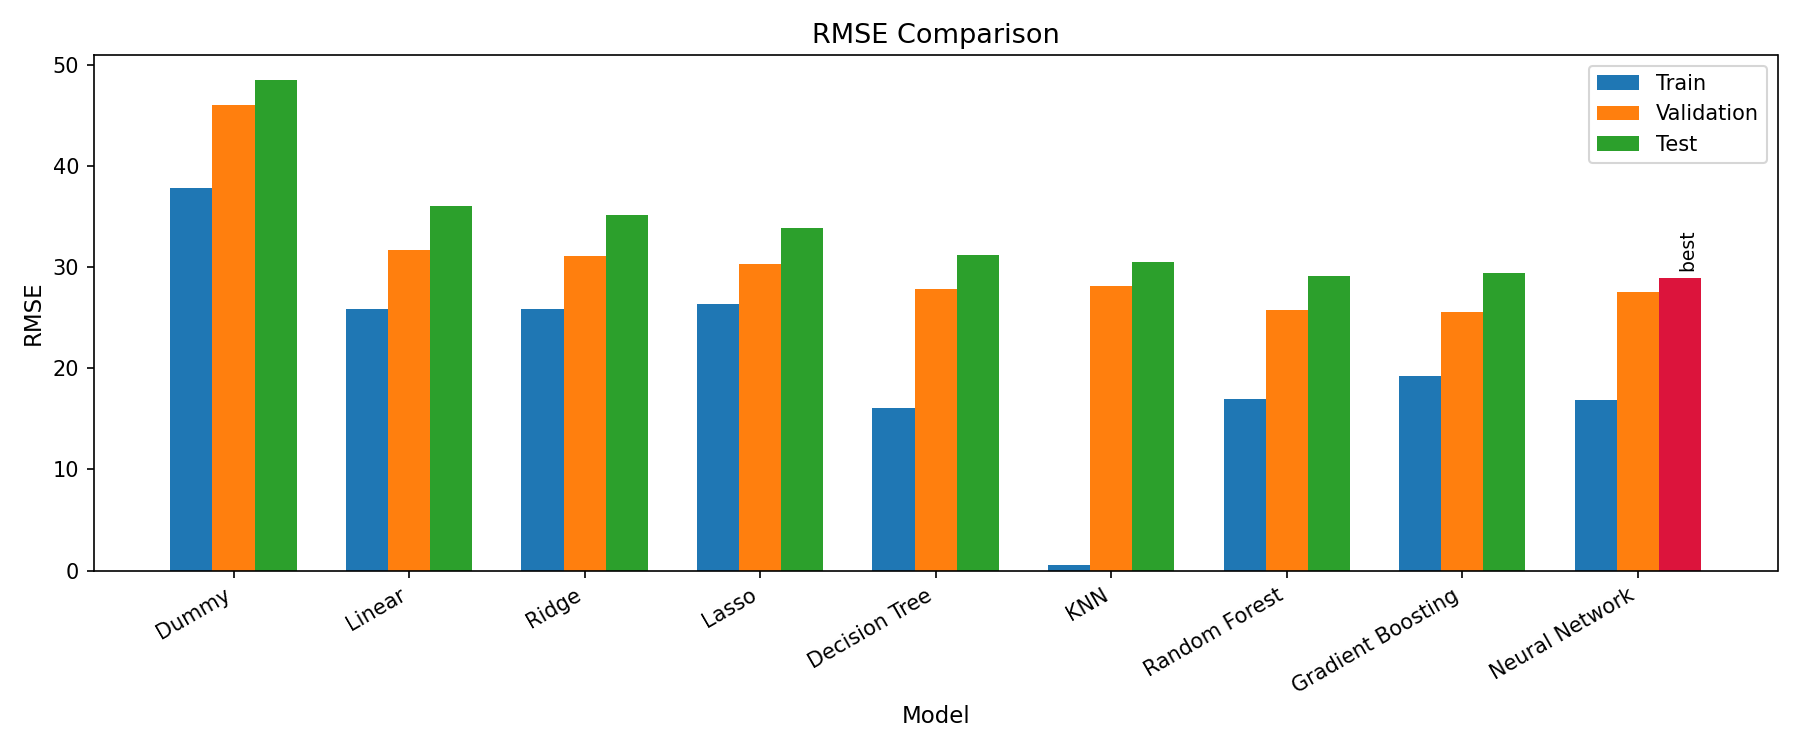
\includegraphics[width=\textwidth]{rmse_comparison.png}
    \end{minipage}
    \hfill
    \begin{minipage}{0.49\textwidth}
        \centering
        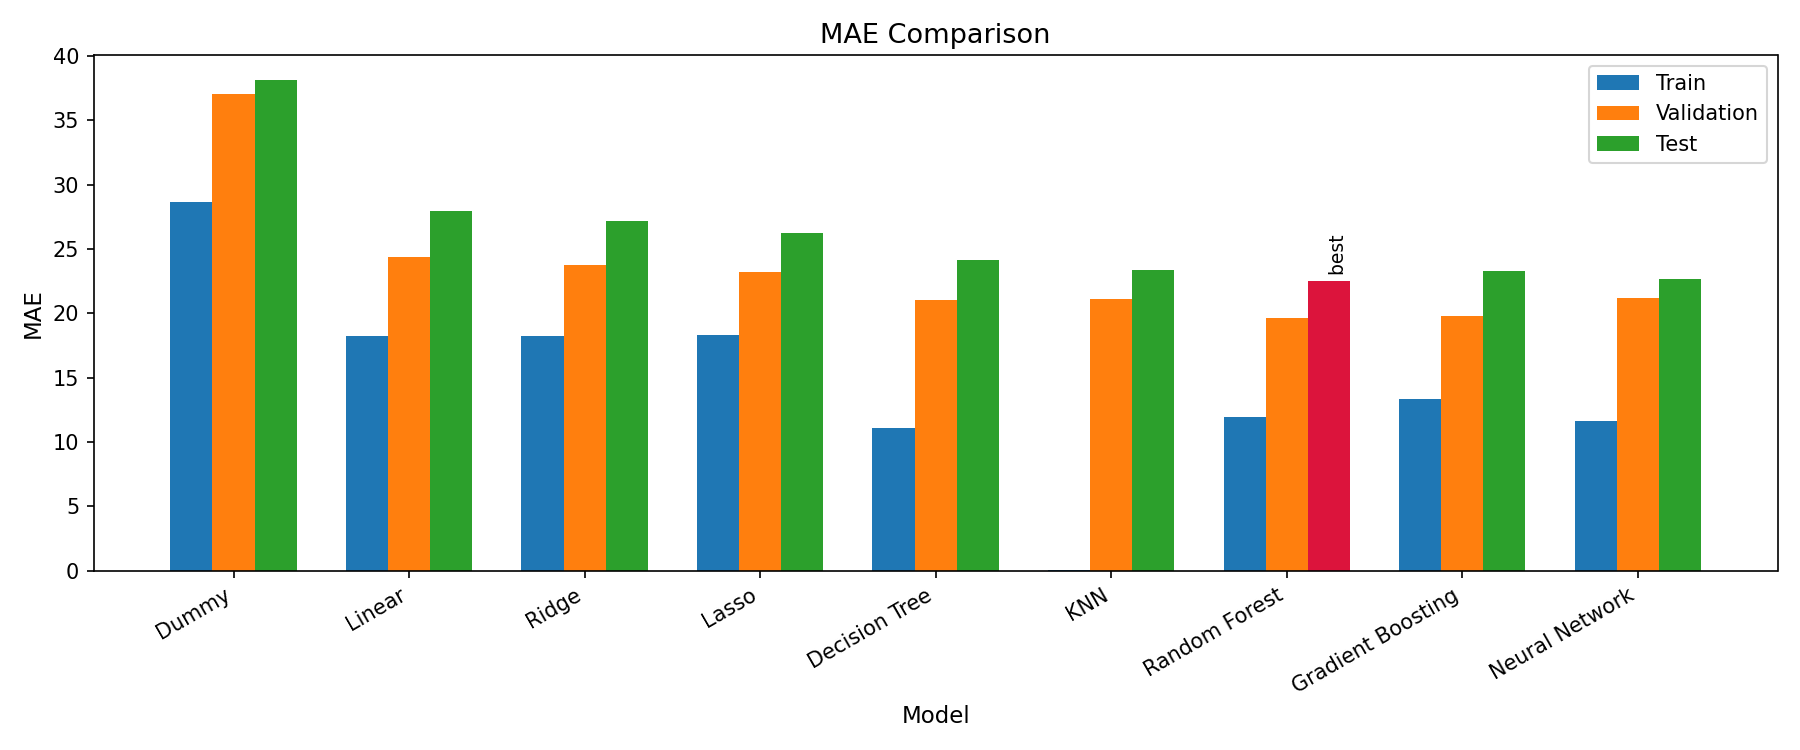
\includegraphics[width=\textwidth]{mae_comparison.png}
    \end{minipage}
    \caption{RMSE and MAE comparison across train, validation, and test splits. These plots show that ensemble trees reduce error substantially compared with the baseline and the linear models.}
    \label{fig:error-main}
\end{figure}

\begin{figure}[H]
    \centering
    \begin{minipage}{0.49\textwidth}
        \centering
        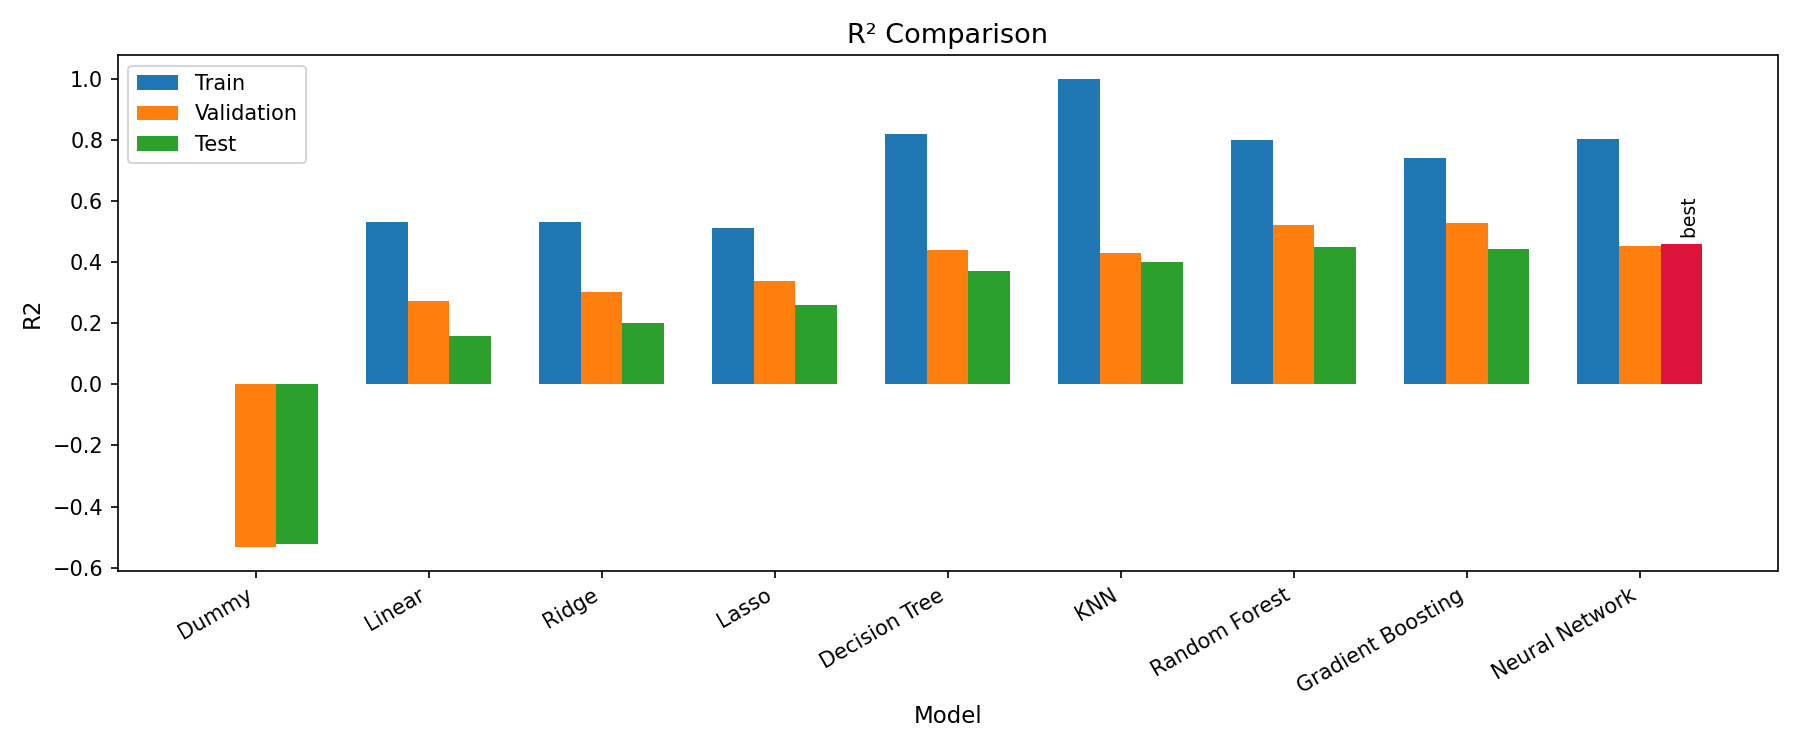
\includegraphics[width=\textwidth]{r2_comparison.png}
    \end{minipage}
    \hfill
    \begin{minipage}{0.49\textwidth}
        \centering
        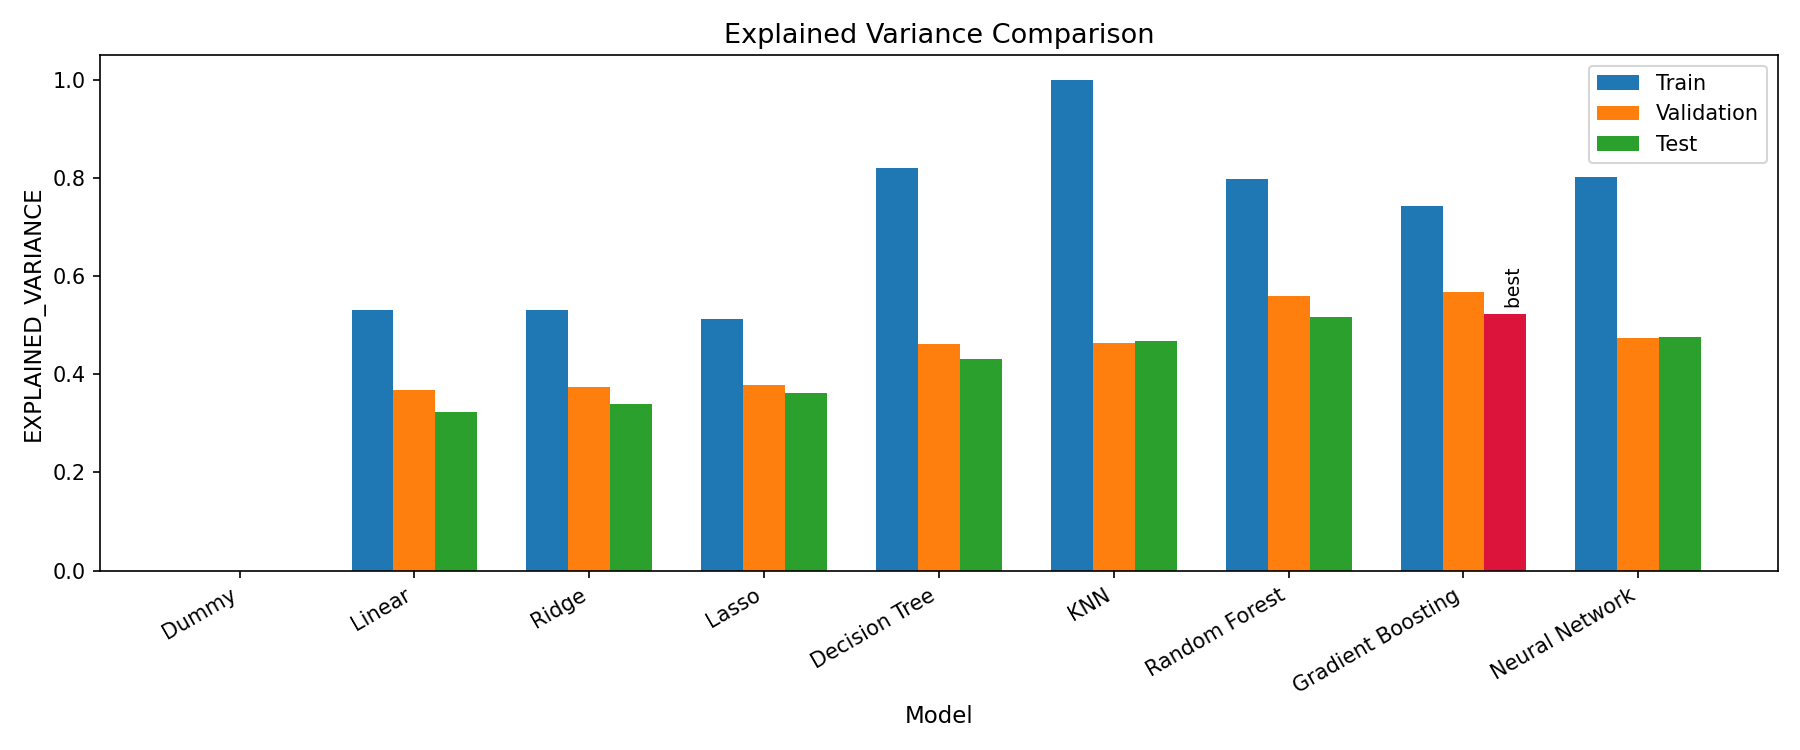
\includegraphics[width=\textwidth]{explained_variance_comparison.png}
    \end{minipage}
    \caption{$R^2$ and explained variance comparison. The same pattern appears in both views: the ensemble models explain the largest share of the target variation.}
    \label{fig:variance-metrics}
\end{figure}

\begin{figure}[h]
    \centering
    \begin{minipage}{0.49\textwidth}
        \centering
        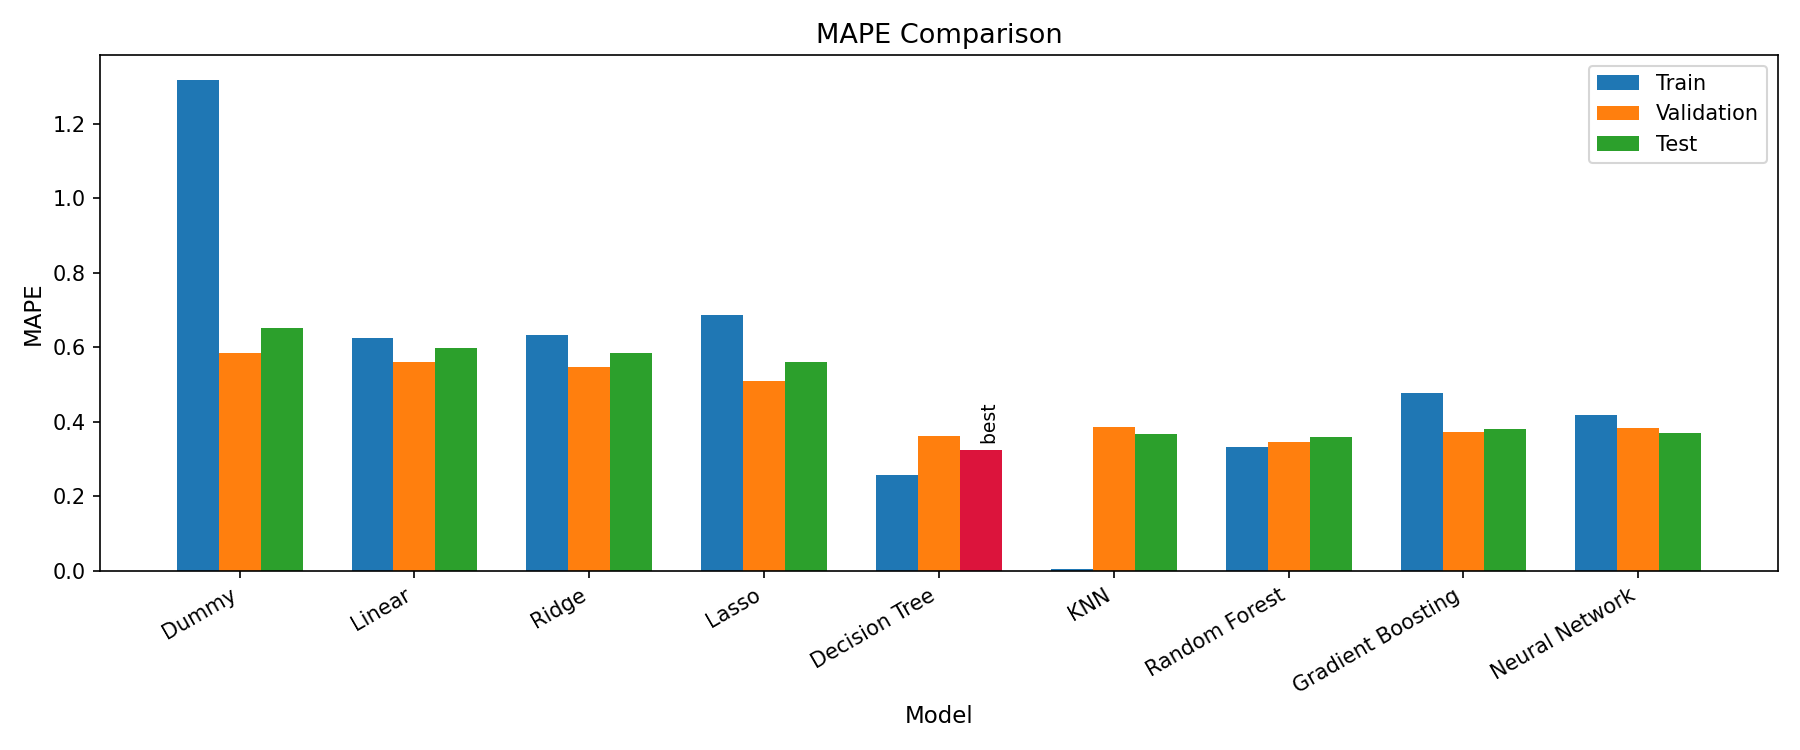
\includegraphics[width=\textwidth]{mape_comparison.png}
    \end{minipage}
    \hfill
    \begin{minipage}{0.49\textwidth}
        \centering
        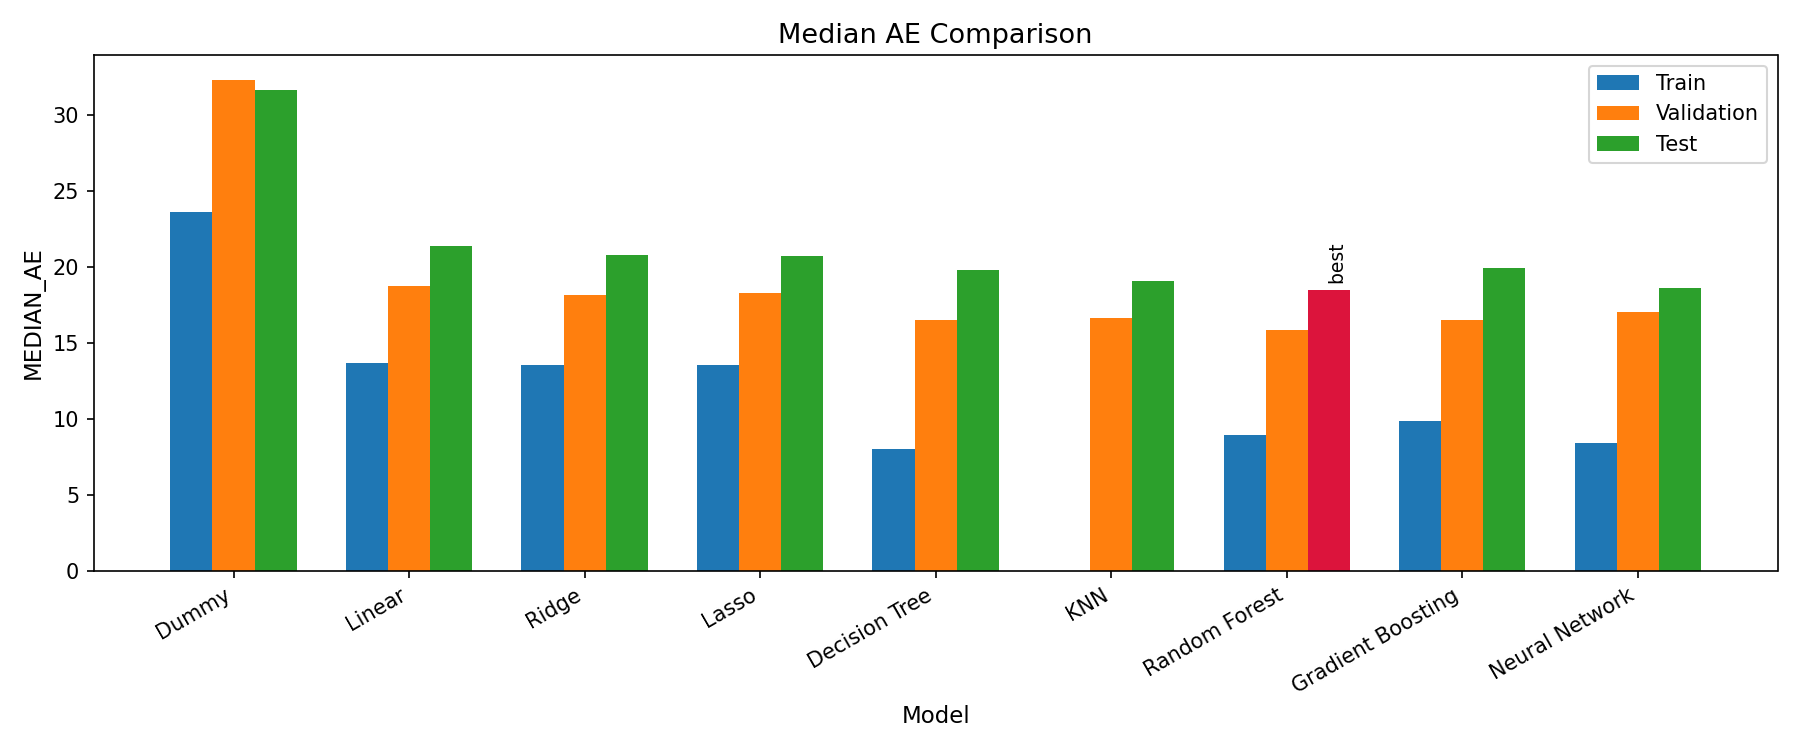
\includegraphics[width=\textwidth]{median_ae_comparison.png}
    \end{minipage}
    \caption{MAPE and median absolute error. These metrics support the same overall conclusion, while also showing that some models differ in how stable their typical errors are.}
    \label{fig:robust-metrics}
\end{figure}

\begin{figure}[h]
    \centering
    \begin{minipage}{0.49\textwidth}
        \centering
        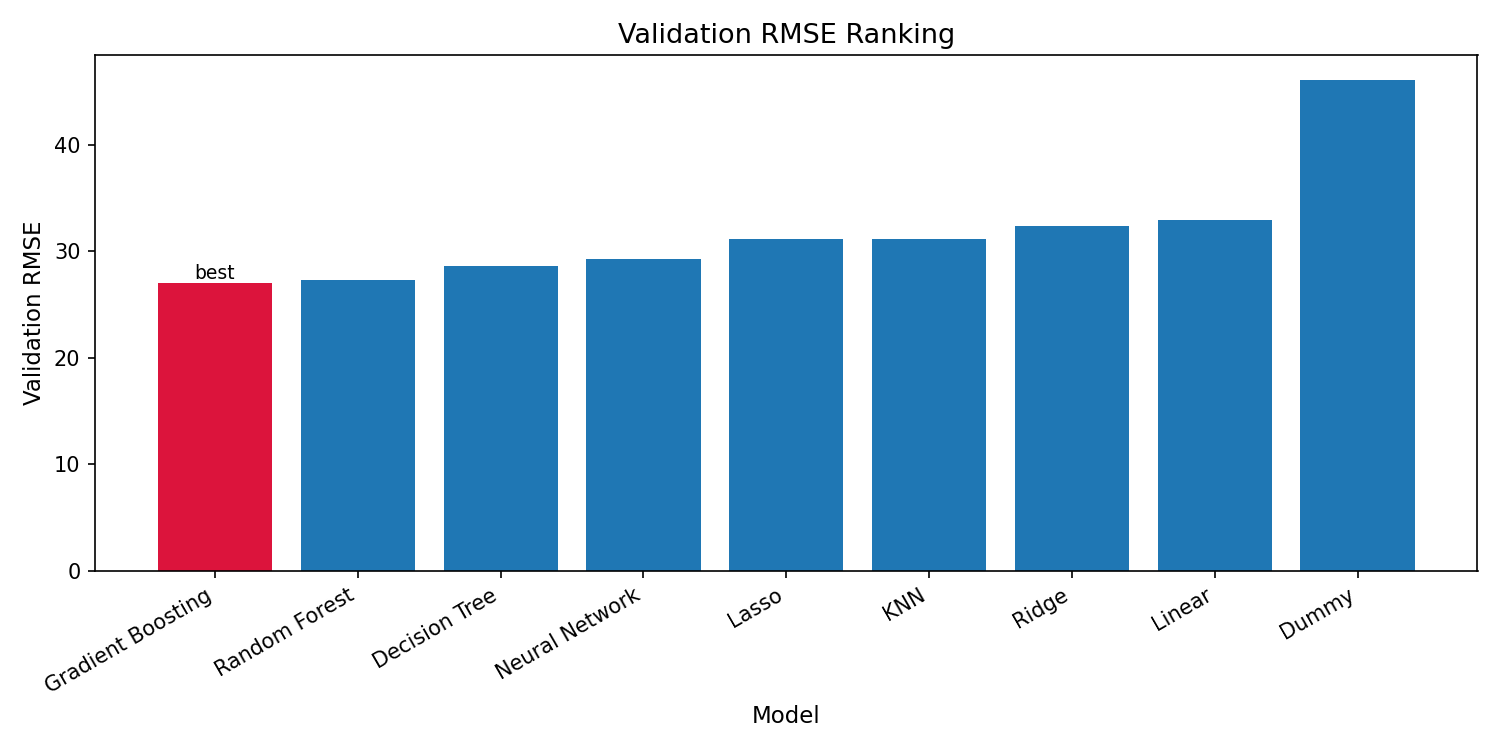
\includegraphics[width=\textwidth]{validation_rmse_ranking.png}
    \end{minipage}
    \hfill
    \begin{minipage}{0.49\textwidth}
        \centering
        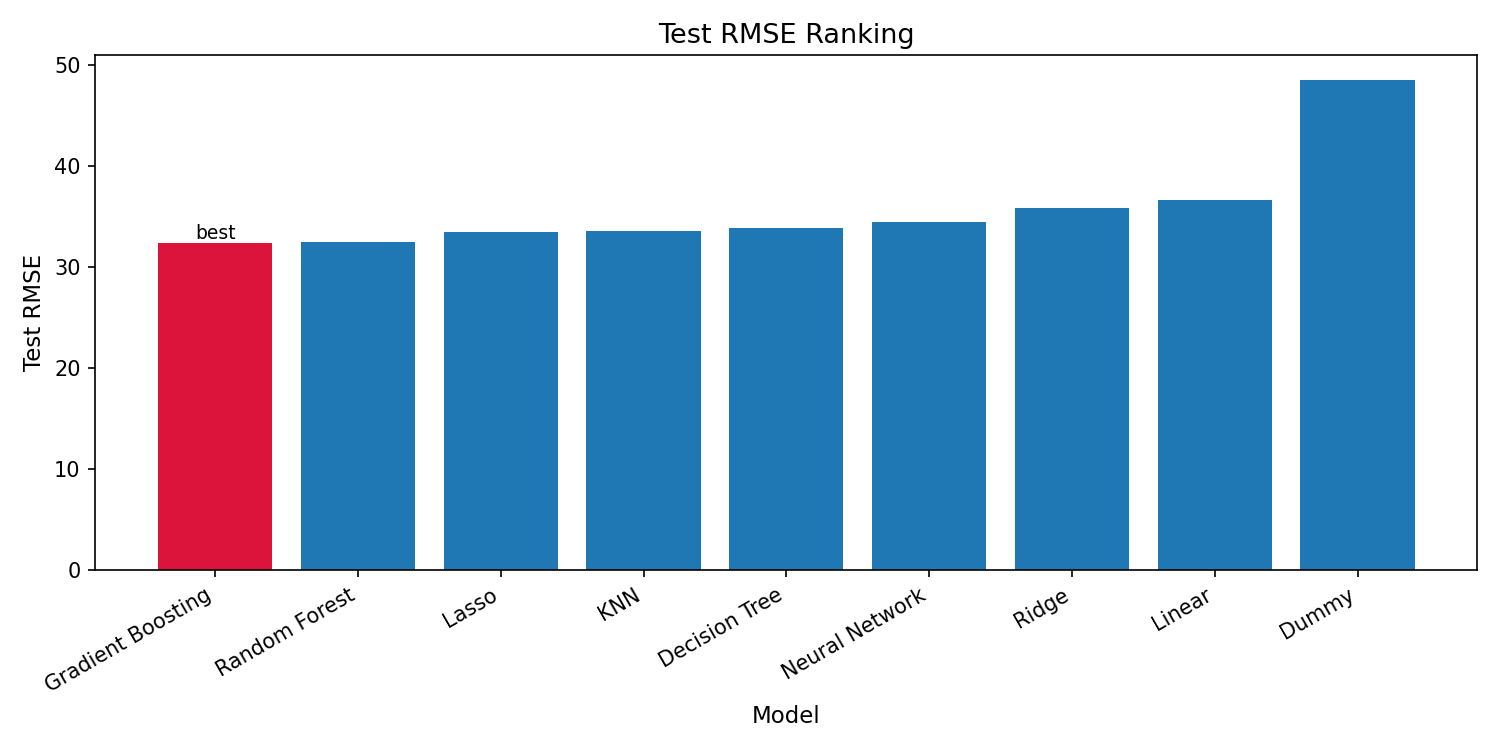
\includegraphics[width=\textwidth]{test_rmse_ranking.png}
    \end{minipage}
    \caption{Ranking by validation RMSE and test RMSE. Gradient Boosting wins the validation phase, but Random Forest becomes the best model on the final test set.}
    \label{fig:rmse-rankings}
\end{figure}

\begin{figure}[h]
    \centering
    \begin{minipage}{0.49\textwidth}
        \centering
        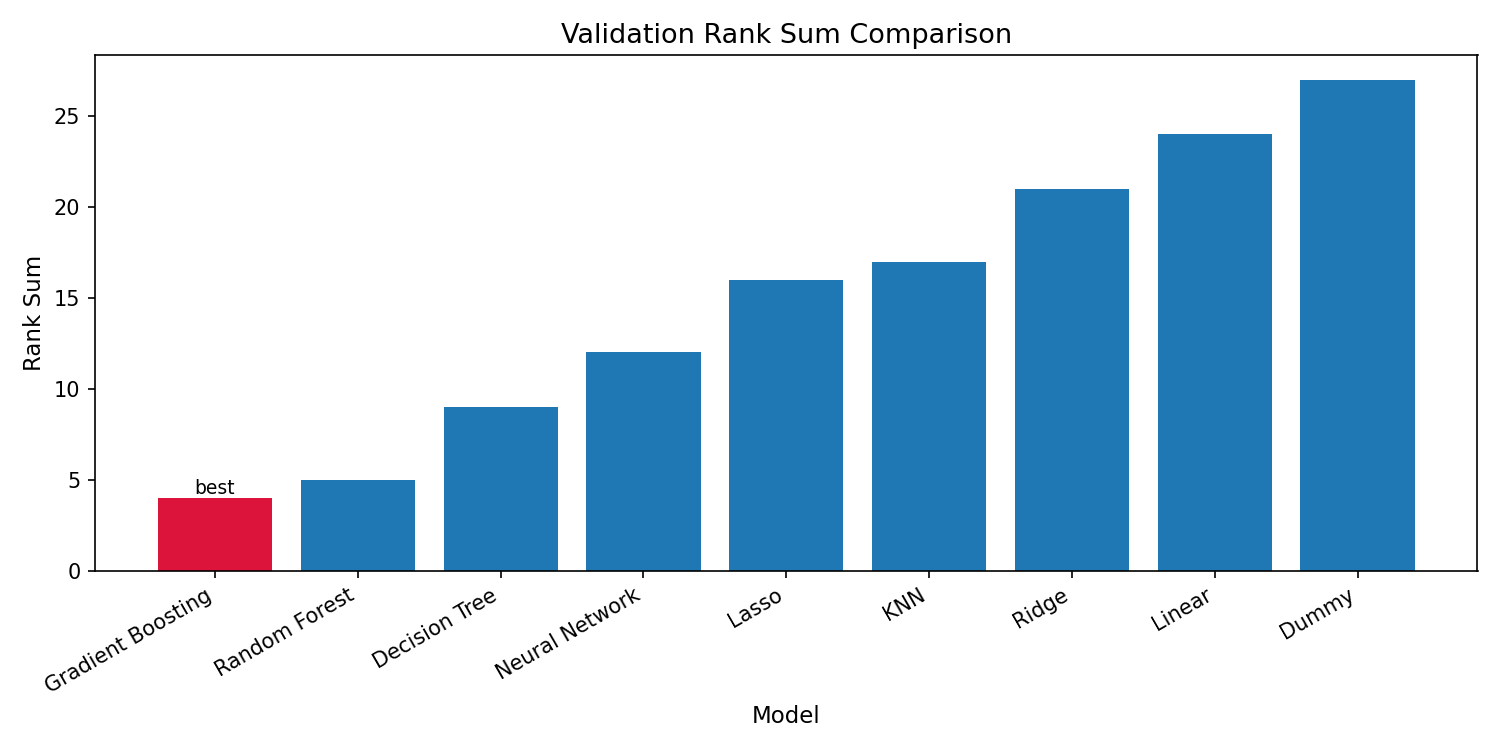
\includegraphics[width=\textwidth]{validation_rank_sum.png}
    \end{minipage}
    \hfill
    \begin{minipage}{0.49\textwidth}
        \centering
        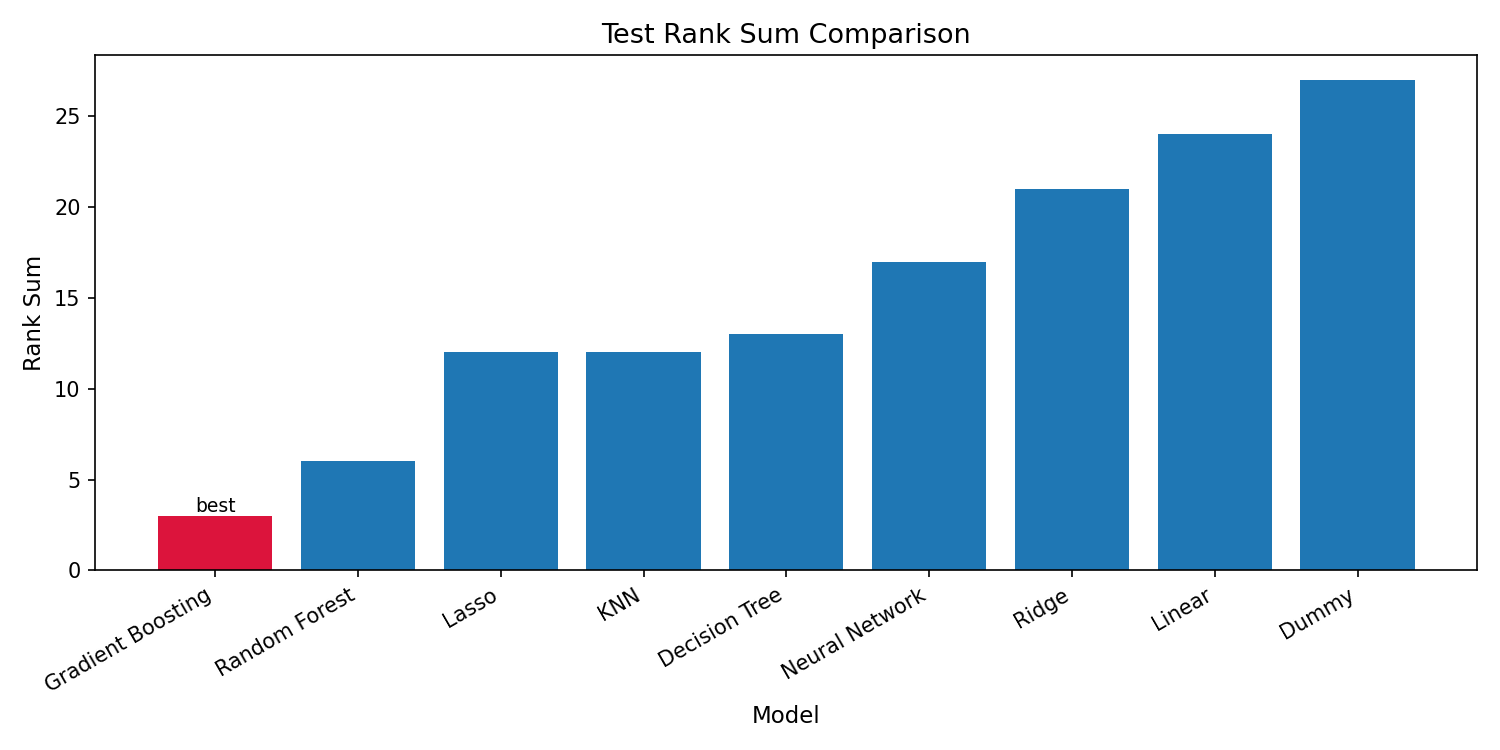
\includegraphics[width=\textwidth]{test_rank_sum.png}
    \end{minipage}
    \caption{Rank-sum comparison across multiple metrics. This gives a broader summary than a single metric and again shows Gradient Boosting on top for validation and Random Forest on top for the final test comparison.}
    \label{fig:rank-sum}
\end{figure}

\section{Interpretation of the Current Results}
The model comparison leads to several important conclusions.

First, the feature engineering work clearly mattered. The large gap between Dummy and the real models 
shows that the final reduced dataset is not arbitrary. It contains useful signal from weather, time, 
and station-related information.

Second, the improvement path across model families is informative. The move from Linear to Ridge and 
then to Lasso shows that regularization is helpful, but the gains stay limited. This suggests that the 
main remaining challenge is not simply coefficient instability. The problem likely contains nonlinear 
interactions and station-specific effects that linear models cannot capture well.

Third, the tree-based models confirm this interpretation. Decision Tree already improves strongly over 
the linear family, and the ensemble versions improve even more. This strongly suggests that the demand 
process includes nonlinear behaviour. Examples that fit this pattern are threshold effects in weather, 
different station sensitivities, and interactions between season, daylight, and rain.

Fourth, the current comparison also reveals that model selection depends on the evaluation stage. 
Gradient Boosting is best on validation, which means it was the strongest candidate during development. 
Random Forest is best on the final held-out test set, which makes it the most convincing model at the 
current stage if one model must be selected for reporting. This is an important distinction: the best 
development score and the best final score do not have to be the same.

\section{Direct Weaknesses Visible in the Current Setup}
Even though the results are promising, the current system still has important weaknesses. 
These weaknesses are not small details; they directly explain why the performance is still moderate 
and why the report should remain critical.

The first weakness is the representation of \texttt{start\_station\_id}. In the final reduced table it 
is still treated as a numeric variable. However, a station identifier is not a true numeric quantity. 
There is no meaningful distance between station IDs, and a linear model may interpret the values in a 
way that does not match reality. This is especially problematic for the linear family. The current 
representation is practical, but not ideal.

The second weakness is the simplified daily aggregation. Daily modelling is easier to manage and useful
for a first pipeline, but it removes many short-term demand patterns. Bike rental demand often depends
on commuting peaks, hour-specific weather changes, or short event windows. Aggregating everything at
the day level hides that structure.

The third weakness is the missing lag information. The current predictors do not explicitly include 
yesterday's rentals, last week's rentals, or rolling averages. In a forecasting problem this is a major 
limitation, because rental demand often has temporal dependence. Without lag features, the model only 
sees contemporaneous weather and calendar information and cannot directly use short-term memory.

The fourth weakness is the limited context coverage. The current dataset does not explicitly include 
holidays, public events, road works, local disruptions, transport strikes, or unusual city-specific 
situations in the final modelling file. This means that some strong demand changes remain unexplained. 
The model is then forced to treat them as noise.

The fifth weakness is that the problem is evaluated in a realistic chronological way. This is 
methodologically correct, but it also means the future period may differ from the earlier training 
period. In other words, concept drift is a real issue here. A model that fits the earlier data well 
may still struggle if later behaviour changes.

The sixth weakness is that some models already show a clear train-validation gap. KNN is the strongest 
example: the training fit is extremely strong, but the validation and test results are much worse. 
This is a typical sign of overfitting or overly local memorization. Decision Tree also shows the same 
basic pattern, though less extremely. The linear family shows the opposite tendency: it is safer but 
also more limited, which suggests underfitting relative to the more flexible ensemble methods.

\section{Long Critical Reflection and Next Steps}
At this stage, the project has a strong and reproducible structure, but it is not yet a finished
 forecasting solution. The most important insight is that adding models alone is not the main answer. 
 The comparison already includes several fundamentally different approaches: a trivial baseline, linear 
 regression, regularized regression, a single tree, a local neighbourhood method, and two ensemble tree 
 methods. Because the strongest gains appear when moving to models that can capture nonlinear structure, 
 we now know that the task is more complex than a simple linear relationship between weather and total 
 rentals. However, the test scores also show that even the best model still leaves a large part of the 
 variance unexplained. That means the next improvement should probably come more from better 
 representation than from adding yet another algorithm without changing the data.

The first improvement should be a better encoding of station identity. A raw station ID is a convenient
placeholder, but not a meaningful numeric signal. A one-hot representation, target-aware categorical
strategy, or even station-specific models would be more appropriate. The second improvement should
be richer temporal features. Month and weekday are useful, but they still represent time in a rather
simple way. Cyclical encodings, lag variables, rolling means, and demand history from previous days
or weeks would likely provide much more predictive structure. The third improvement should be a
closer residual analysis. The current aggregated plots tell us which model is better overall, 
but they do not yet tell us where the models fail most strongly. Residuals should be analysed 
by station, season, weather regime, and demand level. This can show whether the model fails on 
high-demand peaks, rainy days, winter periods, or a subset of stations.

A fourth next step is to add learning-curve style diagnostics. The current results already hint at 
both phenomena in different places: the linear models appear safer but limited, while KNN and some 
tree models fit the training data much more strongly than the future data. A proper learning-curve 
analysis would make this diagnosis more explicit. A fifth next step is to reconsider whether daily 
aggregation is the right long-term representation. It was a good decision for building the first 
stable pipeline, but hourly modelling may better match the original demand process if the project 
later aims for more precise operational forecasting.

We transformed a raw data problem into a reproducible machine learning pipeline with clear modelling 
decisions and a transparent comparison of multiple approaches. The best current final model is 
Random Forest on the held-out test set, while Gradient Boosting was the strongest development 
model on validation. That is already a meaningful result. At the same time, it
makes it equally clear that the most valuable next progress will likely come from improving the 
data representation, adding temporal memory, and analysing model failures more deeply rather 
than only increasing algorithmic complexity.

\section{Preliminary Ethical Considerations}

Predicting bike rental demand is generally a low-risk machine learning task. However, we still need to consider some ethical and social effects. 

First, we decided to use only the 20 most used start stations. This was necessary to build a stable first model, but it creates a representation bias. By leaving out smaller stations, our model ignores the demand in areas that might already have fewer services. In a real-world system, this could lead to an unfair distribution of bikes, where less popular neighborhoods get even less attention.

Furthermore, the data we use is completely anonymous and grouped by day and station. This means no personal user information is exposed. If we change our model in the future to use hourly data or specific user types (like registered members or casual users), we must keep this strict privacy standard. 

In future steps of this project, we should also think about the social and economic background of the stations. We must make sure that our model does not systematically disadvantage certain parts of the city.

\section{AI Tool Use}
AI tools were used for drafting support, restructuring text, and helping to standardize code and reporting outputs. The final content, decisions, code execution, result interpretation, and critical reflection were reviewed and organized by the authors.

\end{document}
